\section{Empirical Analysis}

\subsection{Data}
For this analysis we used stocks from the S\&P 500 Index. We did not include the full index as we removed stocks that were not included for the whole time period. This simplifies the process, however it can lead to a survivorship bias as the stocks are not truly randomly picked but rather are already a subset of well performing firms. As we used the same data for all different models, namely the robust Bayesian and the Historical expectations based allocation, we deem it appropriate. For the risk-free rate, we use the yield of a 10-year treasure bill and convert it to a daily rate.\\
\\
We analyzed different time ranges and observed the models performances on the more stable post crisis time period as well as a full range time frame that starts in 2005. A good model should perform well under different market conditions and not succumb to higher volatility periods.\\
\\
For the parameters in this paper, we use the same ones as \cite{anderson_cheng_2016}. For risk aversion $(\theta \,=\,1)$.
The model uncertainty aversion is four for the Bayesian robust model $(\tau\,= \,4)$. In the step of updating model probability when a new model is born, we use perfect sharing prior $(\alpha\,=\,1)$.

\subsection{Benchmark models}
As our benchmark we chose to compare the model to an asset allocation strategy that uses historical expectations as a direct measurement for future asset allocations as well as a simple equal weighted strategy. The historical expectations model assumes that future means and variance are approximated by their full past. This model is non-Bayesian and does not include prior information. All past information is treated as equal. The model can be described as follows.
\begin{align*}
E(R_{t+1}|F_t) &= \hat{\mu}_t \text{ and } V(r_{t+1} |F_t ) = \hat{\Sigma}_t \text{, where}\\
\hat{\mu}_t &= \frac{1}{t}\sum_{s=1}^{t}R_s, \\
\hat{\Sigma}_t &= \frac{1}{t-1}\sum_{s=1}^{t}(R_s-\hat{\mu}_t)(R_s-\hat{\mu}_t)'
\end{align*}
Using this method to calculate the mean and covariance, the actual portfolio weights are computed based on the regular Markovitz mean-variance portfolio optimization approach where he aims to maximize 
\begin{align*}
E(\phi'R_{t+1} + R_ft+1 | F_t)-\frac{\theta}{2}V(\phi' R_{t+1} + R_ft+1 | F_t)
\end{align*}
where $R_ft+1$ denotes the risk free rate of return. We evaluated the models both with constant risk free rate and time-dependent risk free rate and got very similar results. The numbers outlined below are calculated with a time-dependent risk-free rate of return. $\theta$ is a risk aversion parameter. \\
This yields the following optimal portfolio weights:
\begin{align*}
\phi_t &= \frac{1}{\theta} \hat{\Sigma}_t^{-1}\hat{\mu}_t &\text{Historical expectations model}\\
\phi_t &= \Big(\frac{1}{n}\Big)\bf{1} &\text{1/N model}
\end{align*}

\subsection{Evaluation measure}
This paper uses sharpe ratio to evaluate the out-of-sample performance of the portfolio. The sharpe ratio is obtained by dividing the mean excess return of portfolio by its standard deviation. 
$$\frac{\bar{E}(R_{pt+1})}{\bar{\sigma}(R_{pt+1})}$$
$R_{pt+1}$ is portfolio excess return at time t+1. $R_{t+1}$ is individual asset excess return at time t+1. $R_{pt+1}$ can be obtained by the multiplication of weight allocated at date t and the excess return at t+1. $R_{pt+1}\,=\,\phi_{t}^{\prime}R_{t+1}$\\
The time-dependent risk free rate of return is calculated using the daily movements of a 10 year T-bill. 

\subsection{Evaluation results}
To evaluate the performance of the robust Bayesian portfolio model we compared its returns and sharpe ratio to the standard non-robust mean variance Markovitz portfolio selection model earlier described as the historical expectations model $\phi_t &= \frac{1}{\theta} \hat{\Sigma}_t^{-1}\hat{\mu}_t$ and the equally weighted model that simply weights all assets with $\phi_t &= \Big(\frac{1}{n}\Big)\bf{1}$. \\

\begin{center}
\begin{tabular}{l c c c c}
\textbf{Metric} & \textbf{Time Frame}  &\textbf{Equally weighted} & \textbf{std. Markovitz} & \textbf{Robust Bayesian}\\ 
\hline
ann. sharpe ratio &05-12 & 0.00802
 & -0.0014
 & 0.00915 \\ 
cumulative returns &05-12 & 0.19109
 & -0.03256
 & 0.22016 \\  
Lowest return &05-12 & -0.08994
 & -0.08087
 & -0.093974675 \\
25\% percentile return
&05-12 & -0.00648
 & -0.00713
 & -0.00725 \\
50\% percentile return &05-12 & 0.00056
 & 0.000429
 & 0.000185 \\
75\% percentile return &05-12 & 0.00687
 & 0.00754
 & 0.00774 \\
Highest return &05-12 & 0.11353
 & 0.10401
 & 0.10480 \\
\hline
ann. sharpe ratio & 12-20 & 0.06283 & 0.05790
 & 0.04325 \\ 
cumulative returns & 12-20 & 0.80254 & 0.81403 & 0.59229 \\ Lowest return & 12-20 & -0.04312 & -0.04561 & -0.04320 \\
25\% percentile return & 12-20 & -0.00373 & -0.00400
 & -0.00419 \\
50\% percentile return & 12-20 & 0.00054 & 0.00054 & 0.00029 \\
75\% percentile return & 12-20 & 0.00533 & 0.00613 & 0.00583 \\
Highest return & 12-20 & 0.03098 & 0.03588 & 0.03688  \\
\hline
\end{tabular}
\caption{Summary Statistics with 30 assets portfolio 100 periods rolling window (no short-selling)}
\end{center}

\begin{table}[h]
\begin{center}
\begin{tabular}{l c c c c}
\textbf{Metric} & \textbf{Timeframe} & \textbf{Equally weighted} & \textbf{std. Markovitz} & \textbf{Robust Bayesian}\\ 
\hline
ann. sharpe ratio & 05-12 & 0.00802
 & -0.00241
 & 0.01194 \\ 
cumulative returns & 05-12 & 0.19109
 & -0.06285
 & 0.32455 \\  
Lowest return & 05-12 & -0.08994
 & -0.11561
 & -0.10405 \\
25\% percentile return & 05-12 & -0.00648
 & -0.00840
 & -0.00848 \\
50\% percentile return & 05-12 & 0.00056
 & -0.00008
 & -0.00007 \\
75\% percentile return & 05-12 & 0.00687
 & 0.00857
 & 0.00922 \\
Highest return & 05-12 & 0.08033
 & 0.08033
 & 0.14091 \\
\hline
ann. sharpe ratio & 12-20 & 0.06283 & 0.02710 & 0.02813 \\
cumulative returns & 12-20 & 0.80254 & 0.44596 & 0.44965 \\
Lowest return & 12-20 & -0.04312 & -0.05478 & -0.04718 \\
25\% percentile return & 12-20 & -0.00373 & -0.00572
 & -0.00560 \\
50\% percentile return & 12-20 & 0.00054 & 0.00003 & 0.00029 \\
75\% percentile return & 12-20 & 0.00533 & 0.00708 & 0.00699 \\
Highest return & 12-20 & 0.03098 & 0.04339 & 0.03919  \\
\hline
\caption{Summary Statistics with 30 assets portfolio 100 periods rolling window (with short-selling)}
\end{tabular}
\end{center}
\end{table}
During year 2005 to 2010, both sharpe ratio and cumulative return show that Bayesian model cannot outperform the other two. The equally weighted strategy has the highest sharpe ratio and cumulative return, and it has the lowest volatility among three strategies. Both standard Markovitz and Bayesian model have a negative cumulative return, indicating that they underperform risk-free rate in this time frame. \\
\\
However, an interesting phenomenon happens from October 2008 to March 2009 (See Figure 1 and Figure 2). It is well known that on September 15 2008, the bankruptcy of Lehman Brothers triggered global panic. Economies nearly collapsed during this period, and governments, central banks, and Federal Reserve cooperated together to save the economy. During this period, Bayesian model has a better performance than the other two. While equally weighted and non-robust mean variance strategies are struggling with negative sharpe ratios, Bayesian model is in the positive domain. A possible explanation could be that, during crisis period, prior information is very important since a stock has negative return yesterday may trigger more investors to sell it today. Bayesian model has a storage of prior information which could be a possible reason why it beats the other two models. This could serve as an evidence that Bayesian model perform better during financial crisis. However, it is arbitrary to reach a conclusion and further evaluation need to be performed.\\
\\
During more the stable years 2010 to 2015 robust Bayesian was able to outperform std. Markovitz in terms of sharpe ratio and cumulative returns while having a smaller drawdown, however itself got outperformed by the simple equally weighted strategy in all of these metrics besides drawdown which the equally weighted shows the biggest. These mixed results show that now clear winner emerges and that depending on time period and evaluation metric one might outperform the other. In any case all of the models are similar to each other, both in terms of magnitude and sign. 

\begin{figure}[h]
    \centering
    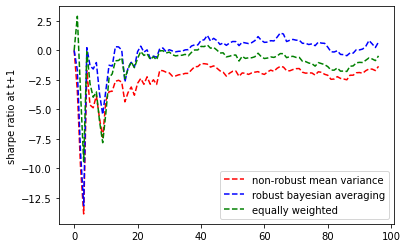
\includegraphics[width=0.75\textwidth]{Images/sharpe.png}
    \caption{sharpe-ratio at t+1 from October 2008 to March 2009}
    \label{fig:mesh1}
\end{figure}

\begin{figure}[h]
    \centering
    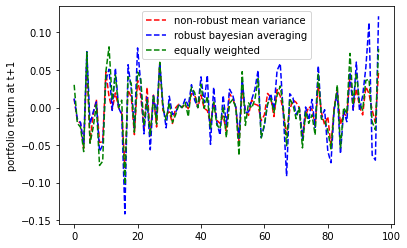
\includegraphics[width=0.75\textwidth]{Images/return.png}
    \caption{portfolio return at t+1 from October 2008 to March 2009}
    \label{fig:mesh1}
\end{figure}

During the most recent five years, the performance of the three strategies mirrored the behaviour of the earliest time frame. Robust Bayesian was outperformed by both other strategies and yielded a disastrous return, considering that the period saw two major equity rushes. Fair to say, that it also saw a major equity sell-off. The robust Bayesian strategy seems to be the most conservative in this period, since the lowest return is the highest among the three strategies and it has a small variance.

To test the robustness of these results we also tested it on a separate data set. This data represents the typical swiss pension funds asset classes and is entirely comprised of different indices and bonds. It is monthly data set starting in 1960 and ending in 2020. The results of this additional analysis are summarized in the following table. With this data the robust Bayesian model clearly outperforms the others, which is somewhat surprising, given that the inputed data is generally considered to be less risky and volatile than the previously tested stock data. Also of note is that the results for the equally weighted approach and the std. Markovitz approach are identical, indicating that with such few stocks the model ends up allocating as the equally weighted method. 
\begin{center}
\begin{tabular}{l c c c c}
\textbf{Metric} & \textbf{Timeframe} & \textbf{Equally weighted} & \textbf{std. Markovitz} & \textbf{Robust Bayesian}\\ 
\hline
ann. sharpe ratio & 1960-2020 & 1.72765 & 1.72765 & 2.38331 \\
cumulative returns & 1960-2020 & 1.93389 & 1.93389 & 4.35451 \\
Lowest return & 1960-2020 & -0.14934 & -0.14934 & -0.22996 \\
25\% percentile return & 1960-2020 & -0.007892 & -0.007892 & -0.008979 \\
50\% percentile return & 1960-2020 & 0.003534 & 0.003534 & 0.004137 \\
75\% percentile return & 1960-2020 & 0.01672 & 0.01672 & 0.02433 \\
Highest return & 1960-2020 & 0.1007 & 0.1007 & 0.0.2858  \\
\hline
\caption{Indices data}
\end{tabular}
\end{center}

\begin{figure}[H]
We find that the Bayesian model only uses the last couple of time steps as informative inputs. After a short amount of time the probability of earlier models converges to zero. Exemplary some the probability of some priors are presented in the following figures. One can see that most often the most recent model is assigned the most weight and that after about 5 time steps no weight is assigned to earlier models at all. This indicates that the stocks do not have extensive "memories" which is part of the reason why modeling future behaviour and trends is generally very difficult.
\minipage{0.32\textwidth}
  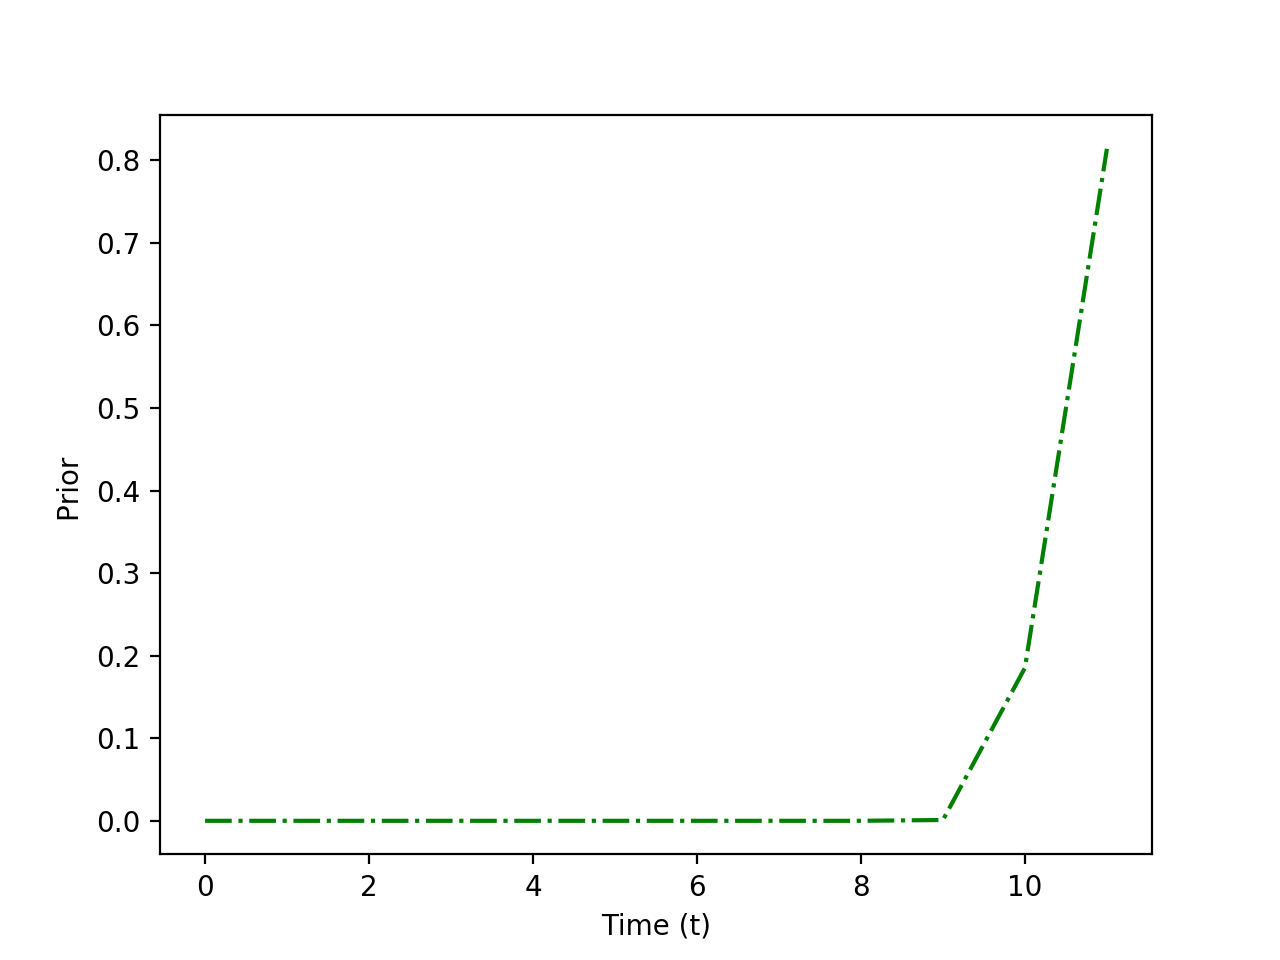
\includegraphics[width=\linewidth]{Images/Figure_prior.png}
  \caption{Bayesian Prior 1}\label{fig:awesome_image1}
\endminipage\hfill
\minipage{0.32\textwidth}
  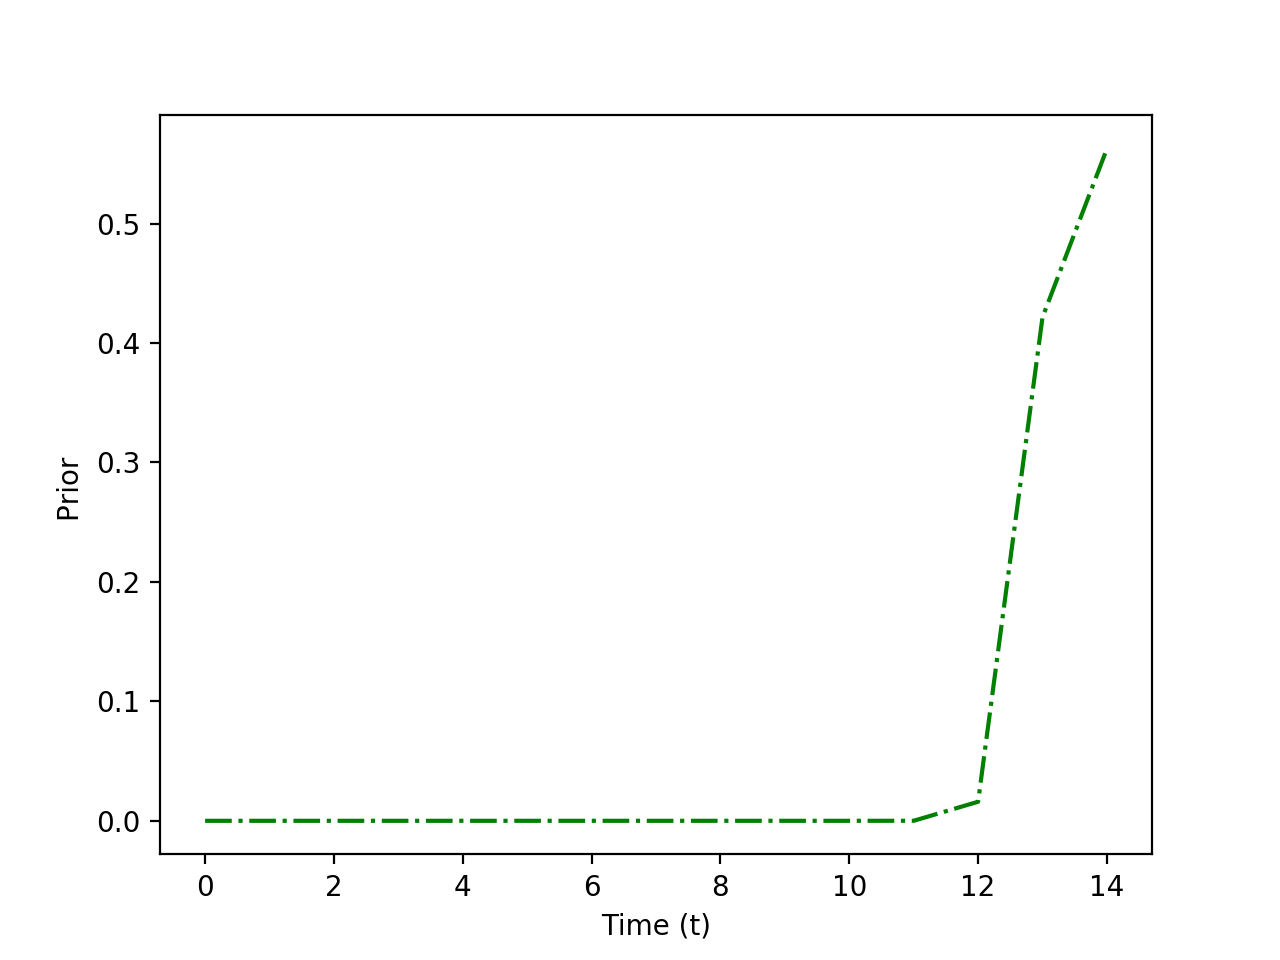
\includegraphics[width=\linewidth]{Images/Figure_prior2.png}
  \caption{Bayesian Prior 2}\label{fig:awesome_image2}
\endminipage\hfill
\minipage{0.32\textwidth}%
  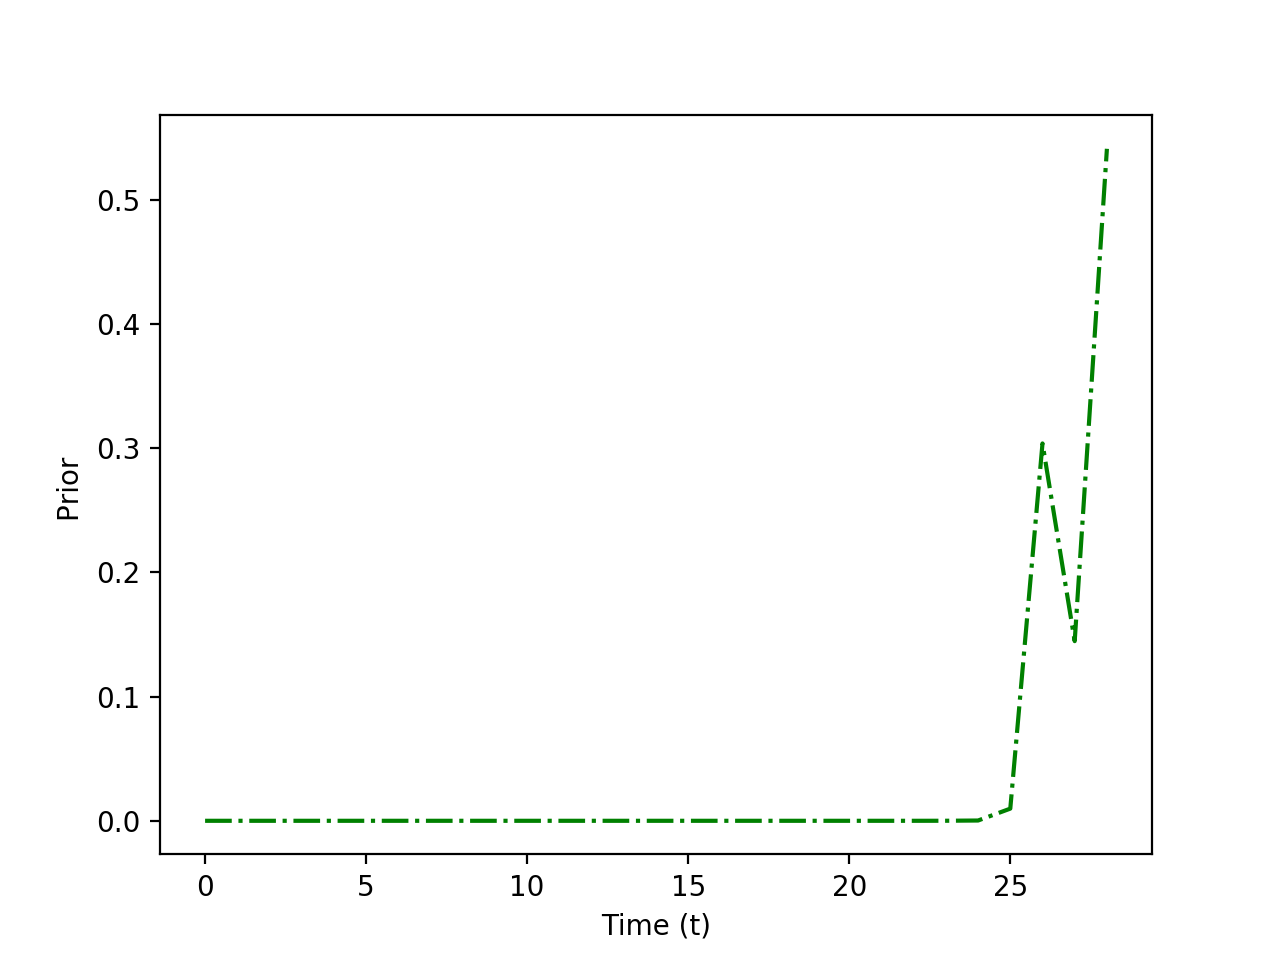
\includegraphics[width=\linewidth]{Images/Figure_prior3.png}
  \caption{Bayesian Prior 3}\label{fig:awesome_image3}
\endminipage
\end{figure}

